\documentclass[a4paper]{article}
\usepackage{graphicx}
\graphicspath{ {./img/} } % Required for inserting images
\usepackage[czech]{babel}
\usepackage[T1]{fontenc}
\usepackage[utf8]{inputenc}
\usepackage[top=1.5 cm, left=1.5 cm, right=15mm, bottom=15mm]{geometry}
\usepackage{fancyhdr, color, multicol}
\usepackage{ragged2e}
\usepackage{blindtext}
\usepackage{lipsum}
\usepackage{multicol}
\usepackage{tikz}
\usepackage{color}
\usepackage[fontsize=12pt]{fontsize}
\usepackage{circuitikz} %obvody, znacky
\usetikzlibrary{arrows}
\usepackage{tkz-euclide}
\usepackage{hyperref}
\hypersetup{
    colorlinks=true, %set true if you want colored links
    linktoc=all,     %set to all if you want both sections and subsections linked
    linkcolor=black,  %choose some color if you want links to stand out
}
%==========================Fonts=====================================
\usepackage{lmodern}
\rmfamily
\DeclareFontShape{T1}{lmr}{b}{sc}{<->ssub*cmr/bx/sc}{}
\DeclareFontShape{T1}{lmr}{bx}{sc}{<->ssub*cmr/bx/sc}{}
%====================================================================
\begin{document}
\thispagestyle{empty}
\begin{center}
    \vspace*{5cm}
    {\huge{1. Architektura PC}} \par
    \vspace{15cm}
    {\large{lilman2727}}
\end{center}


\newpage
\thispagestyle{empty}
\tableofcontents
\newpage

\section{Velice stručná historie}
    \subsection{Analytický stroj}
        Analytický stroj je návrh obecně použitelného mechanického počítače. Obsahoval aritmetickou jednotku, řídící tok s podmíněným větvením a cykly a integrovanou paměť. Je to první \textit{turingovsky úplný} počítač, což znamená, že by teoreticky dokázal vyřešit jakoukoliv úlohu za pomocí přesně definovaných kroků zapsaných přesně definovanými symboly (algoritmem).\par
        S návrhem přišel anglický matematik Charles Babbage v roce 1837. Babbage ho sám nikdy nedokončil. První obecný počítač bude postaven až po více než 100 letech.

    \subsection{Turingův stroj}
        Turingův stroj je teoretický počítač, popsaný matematikem Alanem Turingem v roce 1936. Stroj posouvá nekonečně dlouhou pásku dle daných pravidel. Stroj z této pásky může číst či do ní zapisovat. Je teoreticky schopen vyřešit libovolný problém podle algoritmu.
    \subsection{Bombe}
        Bombe byl elektromechanický počítač sestrojený Alanem Turingem za druhé světové války. Jeho cílem bylo dešifrovat tajné zprávy zašifrované pomocí německé Enigmy. Stroj jako takový simuloval 36 strojů Enigma, s celkem 108 rotory, každý simulující 1 rotor stroje Enigma. Bombe využil slabinu Enigmy -- vstupní písmeno se nikdy nerovnalo výstupnímu 
    \subsection{ENIAC}
        Z anglického \textit{Electronic Numerical Integrator and Computer} byl první programovatelný elektronkový počítač sestrojený v roce 1945 v USA. Jeho prvním úkolem bylo zjistit proveditelnost termojaderné zbraně. Pro své logické obvody používal elektronky, tedy vakuuové trubičky; takovéto počítače jsou označovány názvem \textit{počítače první generace}. Jeho nástupce, MANIAC byl prvním strojem, který porazil člověka ve hře podobné šachu, tzv. Los Alamos šachy, hrané na $6 \times 6$ šachovnici, tedy bez střelců.
    \subsection{UNIVAC}
        Z anglického \textit{UNIVersal Automatic Computer} byl první komerčně vyráběný počítač. Byl vyrobený v USA a na vývoji se podíleli vynálezci strojů ENIAC a MANIAC. Tento počítač je známý tím, že předpovědel vítězství Eisenhowera ve volbách v roce 1952. Stejně jako ENIAC a MANIAC používal pro své obvody elektronky.
    \subsection{IBM PC}
        Uvedený na trh v roce 1981, tento počítač odstartoval éru počítačů jak je známe dnes. Přinesl uživatelské rozhraní a časem i spoustu rozšiřujících karet. Díky vynálezu mikroprocesoru bylo možné razantně zmenšit velikost počítače -- odstupuje se od sálových počítačů. Dnešní počítače jsou jakýmisi praprapravnuky právě IBM PC, používal procesor Intel 8088, měl paměť RAM a podporoval diskety.

\newpage


\section{Architektura počítačů}
    \textit{Architektura počítače} je způsob realizace počítače. Zaměřuje se na návrh a konstrukci zařízení, která zpracovávají data. Zkoumá, jak pracuje CPU a jak přistupuje k paměti.
    \subsection{Von Neumannova architektura}
        Architektura popsaná americko-maďarským matematikem Johnem von Neumannem. Popisuje počítač, který má společnou paměť pro instrukce i data. Zpracování dat je \textit{sekvenční}, tj. instrukce se vykonají v přesném pořadí jedna za druhou. Von Neumannova architektura  popisuje řadič s aritmeticko-logickou jednotkou jako centrální procesorovou jednotku, která komunikuje s pamětí. \par
        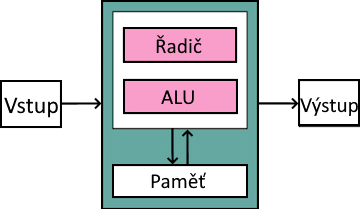
\includegraphics{vonNeumann.png}  
    \subsection{Řadič}
        \textit{Řadič} řídí celou činnost počítače. Řadič v procesoru je nadřazen všem ostatním řadičům (např. paměťový řadič, SATA řadič\dots)
        Počítač řídí pomocí řídících signálů, které zasílá jednolivým modulům počítače a odpovědi na tyto signály jsou předány zpět do řadiče. \par
        V dnešní době používáme tzv. \textit{mikroprogramovatelné řadiče}, tedy řadiče řízené kódem, který je uložený v paměti. \par
        Existují tři typy mikroprogramovatelných řadičů:
        \begin{itemize}
            \item Horizontální -- používá dlouhé mikroinstrukce, které obsahují i řídící signály. Každá mikroinstrukce vyžaduje 1 takt. Mikroinstrukce obsahuje i adresu paměti.
            \item Vertikální -- používá krátké mikroinstruke, které však vyžadují více taktů.
            \item Diagonální -- kompromis mezi horizontálním a vertikálním. Jedna mikrointrukce vyžaduje 1 takt, ale neobsahuje adresu paměti, proto musí být přítomen i programový čítač.
        \end{itemize}
    \subsection{Aritmeticko-logická jednotka}
        \textit{Aritmeticko-logická jednotka}, neboli \textit{ALU} provádí logické (negace, konjunkce, disjunkce \dots) a aritmetické (sčítání, násobení, bitový posun \dots) operace s daty podle programu. ALU se používá výhradně pro celočíselné operace. Pro operace s plovoucí desetinnou čárkou se používá tzv. \textit{FPU}, neboli \textit{FLoating-Point Unit}, v češtině \textit{matematický koprocesor}. \par
        Největší velikost dat, se kterým ALU může pracovat se nazývá \textit{slovo}. Dnešní procesory (na architektuře x86-64) mají velikost slova 64 bitů.
    \subsection{Registry}
        \textit{Registr} je nejrychlejší paměť počítače, slouží pro uložení informace o velikosti jednoho slova. CPU používá registry pro práci s čísly a další zpracovávání informací. ALU a FPU mají své vlastní registry o své vlastní délce slova. Délka slova záleží na architektuře daného procesoru a instruknční sady, kterou procesor disponuje.
    \subsection{Sběrnice}
        \textit{Sběrnice}, anglicky \textit{bus} má za účel zajistit přenos dat a řídících povelů mezi dvěma a více elektronickými zařízeními. Přenos dat se řídí stanoveným protokolem -- určitým postupem jak a které informace si předat. V posledních letech se od sběrnic ustupuje ve prospěch dvoubodových spojů, na kterých, na rozdíl od sběrnice, jsou data přenášena bez potřeby adresy, čímž se uvolní místo pro jiná data, a navíší se tak výkon. Příkladem sběrnice je \textit{USB}, zkratka znamenající \textit{Universal Serial Bus}, či sběrnice \textit{PCI}. Příkladem dvoubodového spoje je moderní \textit{PCIe}.
    \subsection{Centrální procesorová jednotka}
        \textit{Centrální procesorová jednotka}, anglicky \textit{Central Processing Unit}, \textit{CPU} je souhrnné označení pro \textit{ALU, FPU, a řadič}. CPU umí vykonávat strojové instrukce a obsluhovat vstupy a výstupy. Na začátku bylo CPU složeno z mnoha individuálních částí, ale v 70. letech minulého století byly všechny části sloučeny do jednoho integrovaného obvodu. CPU, který má části sloučené do integrovaného obvodu se nazývá \textit{mikroprocesor}.
    \subsection{Harvardská architektura}
        Narozdíl od \textit{von Neumannovy} architektury odděluje Harvardská architektura paměť programu a dat. To znamená, že instrukce a programová data jsou uloženy zvlášť a nesdílí sběrnice. CPU může současně číst instrukci a zároveň přistupovat do paměti dat. Dochází tedy k paralelizaci a tudíž ke zvýšení výkonu oproti sekvenčnímu způsobu přístupu k datům von Neumannovy architektury.
        \par
        Dnešní procesory spojují tyto architektury dohromady. Uvnitř se chovají podle Harvardské architektury - oddělují paměť pro data a pro instrukce, ale zvenku se chovají podle von Neumannovy architektury, protože načítá data i program z hlavní paměti (RAM) najednou.
    \subsection{Mikroarchitektury}
        Představuje způsob, jakým je implementovaná instrukční sada v procesoru. Pro jednu danou instrukční sadu může existovat více mikroarchitektur, např. mikroarchitektura \textit{Zen} a mikroarchitektura \textit{Core} implementují instrukční sady x86-64.
        \par
        Hlavním prvkem mikroarchitektury je \textit{exekuční jednotka}, která zahrnuje ALU, FPU, jednotky pro adresování, jednotky pro předpovídání větvení a \textit{SIMD} (Single Instruction, Multiple Data).

\newpage


\section{Hardware počítače}
    \subsection{Procesor}
        Je \uv{mozek} počítače. Procesor postupně zpracovává jednotlivé instrukce programu. Moderní procesory jsou vyráběny z křemíkového substrátu (wafer). Na substrát jsou naneseny miliony nanoskopických tranzistorů. Procesor, který se dnes používá se nazývá \textit{mikroprocesor}, protože je celý uložený do pouzdra integrovaného obvodu. \par
        Dnes se výrobou procesorů zabývají firmy, z nichž jsou hlavní \textit{AMD, Intel, ARM, Nvidia, Apple, Qualcomm}. Intel je schopen i výroby svých mikroprocesorů, kdežto ostatní výrobci jsou odkázáni na dodavatele, jako například \textit{TSMC}.
        Procesor, který dnes používáme obsahuje krom jádra procesoru i integrovaný rozvaděč tepla, který výrazně napomáhá chlazení.
    \subsection{Chladiče}
        Většina elektrické energie dodávaná polovodičovým součástkám je přeměněna na teplo. Protože by se jednotlivé součástky mohly poškodit, je velmi důležité je adekvátně chladit. U procesorů dle \textit{TDP, Thermal Design Power} lze určit, jak moc \uv{budou hřát} a podle toho zvolit správný chladič. \par
        Chladiče můžeme rozdělit následovně:
        \begin{itemize}
            \item Pasivní chlazení -- teplo generované polovodičem se přesune na, většinou hliníkový, chladič, který si vyměňuje teplo s okolím. Pasivní chladiče se v drtivé většině dělají do $37\,W$, po překročení této hodnoty je skoro nutné přejít na aktivní chlazení.
            \item Aktivní chlazení -- lze rozlišit na:
            \begin{itemize}
                \item Chlazení vzduchem -- větrák fouká čerstvý vzduch do chladiče a tak značně pomáhá s rozptylem tepla. Krom větráku je identický s pasivním chladičem ve funkčnosti i v obecném principu funkčnosti.
                \item Chlazení vodou -- používá kapalinu, která proudí skrze uzavřený okruh přes procesor až k radiátoru, kde si s ním vymění teplo. Lze rozdělit na:
                \begin{itemize}
                    \item AIO -- All-in-one -- obsahuje chladící desku, pumpu, kapalinu, trubičky, radiátor a větráky na radiátor v jednom uceleném balení, \uv{plug and play}
                    \item Custom loop -- Všechny výše uvedené části a k tomu rezervoár (nádrž) si koupíte zvlášť a sestavíte se na míru dle svých požadovaných specifikací. Nutné značné úsilí, je dražší.
                \end{itemize}
            \end{itemize}
            \item Chlazení tekutým dusíkem -- v extrémních případech, tekutý dusík se nalévá přímo na jádro CPU/GPU. Velice nepraktické k dennímu použití, ale lze tak dosáhnout nejlepšího výkonu.
        \end{itemize}
    \subsection{Základní deska}
        \subsubsection{Patice}
        \subsubsection{Čipová sada}
        \subsubsection{Napájecí kaskády}
        \subsubsection{Integrované technologie}
        \subsubsection{Sběrnice, piny a jiné konektory}
    \subsection{RAM}
        \subsubsection{Rozdíly mezi SDR, DDR, QDR}
        \subsubsection{Časování a latence}
    \subsection{Grafická karta}
        \subsubsection{Jádro a VRM}
        \subsubsection{Paměť GPU}
        \subsubsection{Srovnání CPU a GPU}
    \subsection{Disky}
        \subsubsection{HDD}
        \subsubsection{SSD}
        \subsubsection{Archaické disky}
    \subsection{Zdroj}
        \subsubsection{Hodnocení zdrojů}
    \subsection{Rozšiřující karty}
    \subsection{Bedny}

\newpage

\section{Reference}
    \begin{itemize}
        \item \url{https://en.wikipedia.org/wiki/MANIAC_I}
        \item \url{https://en.wikipedia.org/wiki/IBM_Personal_Computer}
        \item \url{https://en.wikipedia.org/wiki/UNIVAC_I}
        \item \url{https://cs.wikipedia.org/wiki/ENIAC}
        \item \url{https://cs.wikipedia.org/wiki/Elektronkov%C3%BD_po%C4%8D%C3%ADta%C4%8D}
        \item \url{https://en.wikipedia.org/wiki/Bombe}
        \item \url{https://cs.wikipedia.org/wiki/Turingovsk%C3%A1_%C3%BAplnost}
        \item \url{https://cs.wikipedia.org/wiki/Turing%C5%AFv_stroj}
        \item \url{https://en.wikipedia.org/wiki/Turing_machine}
        \item \url{https://cs.wikipedia.org/wiki/%C5%98adi%C4%8D}
        \item \url{https://cs.wikipedia.org/wiki/%C4%8C%C3%ADta%C4%8D_instrukc%C3%AD}
        \item \url{https://cs.wikipedia.org/wiki/Architektura_po%C4%8D%C3%ADta%C4%8De}
        \item \url{https://en.wikipedia.org/wiki/Processor_register}
        \item \url{https://cs.wikipedia.org/wiki/Aritmeticko-logick%C3%A1_jednotka}
        \item \url{https://cs.wikipedia.org/wiki/Von_Neumannova_architektura}
        \item \url{https://cs.wikipedia.org/wiki/Sb%C4%9Brnice}
        \item \url{https://cs.wikipedia.org/wiki/PCI-Express}
        \item \url{https://cs.wikipedia.org/wiki/Centr%C3%A1ln%C3%AD_procesorov%C3%A1_jednotka}
        \item \url{https://cs.wikipedia.org/wiki/Harvardsk%C3%A1_architektura}
        \item \url{https://cs.wikipedia.org/wiki/Architektura_po%C4%8D%C3%ADta%C4%8De}
        \item \url{https://cs.wikipedia.org/wiki/Mikroarchitektura}
        \item \url{https://cs.wikipedia.org/wiki/Mikroprocesor}
    \end{itemize}
\end{document}